\documentclass{article}
\usepackage{graphicx}
\usepackage[letterpaper,margin=1in]{geometry}

\title{Homework 4\\CME 211}
\author{Gabriel Buchsbaum}

\begin{document}

\maketitle

\section{Truss class functionality}

The Truss object represents the geometry of a truss, as well as the external 
forces being applied. It can be used to plot the geometry of the truss and
calculate the forces in the beams at static equilibrium. A truss object is
created using two files:

\begin{itemize}
  \item A data file containing the x and y coordinates of the joints, the x
    and y components of external forces at each joint, and identification of if
    the joint is rigidly supported
  
  \item A data file containing the joints each beam is connected to
\end{itemize}

When a new truss object is created, it reads and stores the data in these
files. It also creates a blank array as a placeholder for the results attribute
to avoid errors in print statements.

The forces in static equilibrium are calculated by using the
computeStaticEquilibrium method. The basic idea is to create a system of
equations, with two equations representing each joint (the forces in the x
direction and the forces in the y direction). The variables in the system
of equations are the compression forces in each beam and the two components
of the reaction force at each rigidly supported joint. These equations are
set up to find values of the variables such that all forces at each joint sum
to zero. The system of equations can be represented in matrix form as $Ax = b$,
where $A$ is a square matrix holding the coefficients, $x$ is a vector holding
the variables, and $b$ is a vector holding the constants (i.e. the external
forces applied to the truss). The forces in the beams can be determined by
solving for $x$.

There are two methods used to perform the calculations:

\begin{itemize}
\item computeStaticEquilibrium() \\
  This is the method that is called to perform calculations. It sets up the
  matrix and vector representing the system of equations, and uses a solver
  to determine the resulting forces. It does not take in any arguments, and
  changes the results attribute directly rather than using a return value.

\item trig(b) \\
  This method is used to break the forces in the beams into x and y components
  by finding the displacement in each direction and dividing them by the beam
  length. Its input is a number representing a certain beam (zero indexed to
  avoid unnecessarily adding and subtracting one), and its output is a numpy
  array holding the two components in reference to the first joint listed
  for the given beam.
\end{itemize}

The following process is used to determine the values of the forces:

\begin{enumerate}

\item Identify the number of total joints, rigidly supported joints, and
  beams. Use this information to identify the number of equations (2 for every
  joint) and the number of variables (1 for every beam, 2 for every fixed
  joint). If the number of variables does not equal the number of equations,
  an exception is raised, as the truss is overdetermined or underdetermined.

\item Set up numpy arrays to store the coefficients and their respective
  positions in the system of equations, for the purpose of creating a sparse
  matrix. The data array uses float64 data, while the row and column index
  arrays use int32 data.

\item For each beam, divide its compression force into x and y components.
  Record these as coefficients, and determine the correct position in the matrix
  (i.e. placing them in the row for the x or y equation of the correct joint
  and the column representing their beam). This simultaneously handles both
  ends of the beams (flipping the signs for the second end).

\item Identify the correct places in the equation matrix to put the reaction
  forces. One goes in each column, and they are assigned to the row for the
  requisite joint and direction. All of the coefficients for these are 1.

\item Combine all of this information into a sparse CSR matrix
  (scipy.sparse.csr\_matrix) holding the coefficients in the correct location
  for the system of equations.

\item Compile the external forces into a 1D numpy array (with one position for
  each direction of each joint).

\item Use scipy.sparse.linalg.spsolve to find the values of each force.

\end{enumerate}

The results include both the beam and reaction forces, although the truss
only shows the beam forces when it is converted to a string by print().

\section{Example plot}

\begin{figure}[htb]
  \begin{center}
    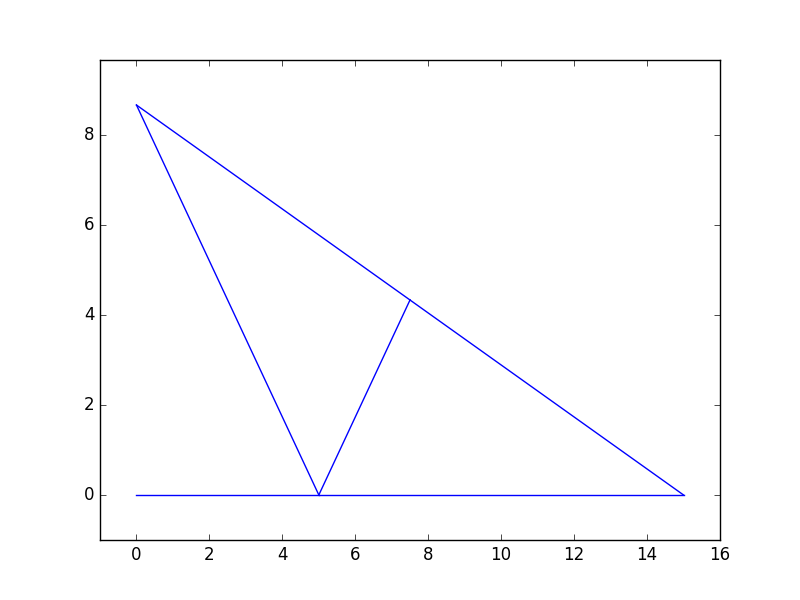
\includegraphics[width=0.75\linewidth]{truss2.png}
    \caption{Truss 2}
    \label{fig:truss2}
  \end{center}
\end{figure}

\end{document}
